\documentclass{article}

%opening
%\usepackage{fullpage}
\usepackage{hyperref}
\usepackage[english]{babel}
\usepackage[utf8]{inputenc}
\usepackage{graphicx}
%\usepackage{amsmath}
\graphicspath{{plots/}}
%\usepackage{listings}

\title{Capita Selecta AI, module 4:\\ Integrating learning and scheduling for an energy-aware scheduling problem}
\author{Tom Decroos \and Daan Seynaeve}

\begin{document}
\maketitle
\begin{abstract}
	We introduce a method to integrate price forecasts into an energy scheduling problem. Rather than focussing on accurate price  predictions, we directly minimize the cost of the resulting scheduling. We present results that show that our approach, which is a relatively simple way of optimizing the pipeline in a holistic way, does not perform better than linear regression on features selected in a sensible way.
	%abstract summary of your findings (1-2 paragraphs)
\end{abstract}
\section{Methods}
%method (overview of scheduling approach,learning approach and their integration)
\subsection{Scheduling approach}
To perform the scheduling, we have have used MiniZinc.

\subsection{Feature selection}
Before training a linear regression model, we first checked the relevance of each feature. The following output from a simple R-script shows the correlation coefficient of all available features.
\begin{verbatim}
> cor(features,prices$SMPEP,use='complete.obs')
prices.HolidayFlag            -0.001837929
prices.WeekOfYear             -0.015813567
prices.DayOfWeek              -0.069624872
prices.PeriodOfDay             0.323490486
prices.ForecastWindProduction -0.079638880
prices.SystemLoadEA            0.491096357
prices.SMPEA                   0.618158287
prices.ORKTemperature         -0.009086615
prices.ORKWindspeed           -0.035435662
prices.CO2Intensity           -0.035055080
\end{verbatim}
We can see that there are only three relevant features for predicting prices: \verb|SystemLoadEA|, \verb|SMPEA| and \verb|PeriodOfDay|. The relation between the first two features and the actual price of electricity is obvious. The relation between \verb|PeriodOfDay| and the actual price is less obvious however. We investigated this further and plotted the average price for each period of the day (Figure \ref{fig:timeslot_average}).

\begin{figure}
	\centering
	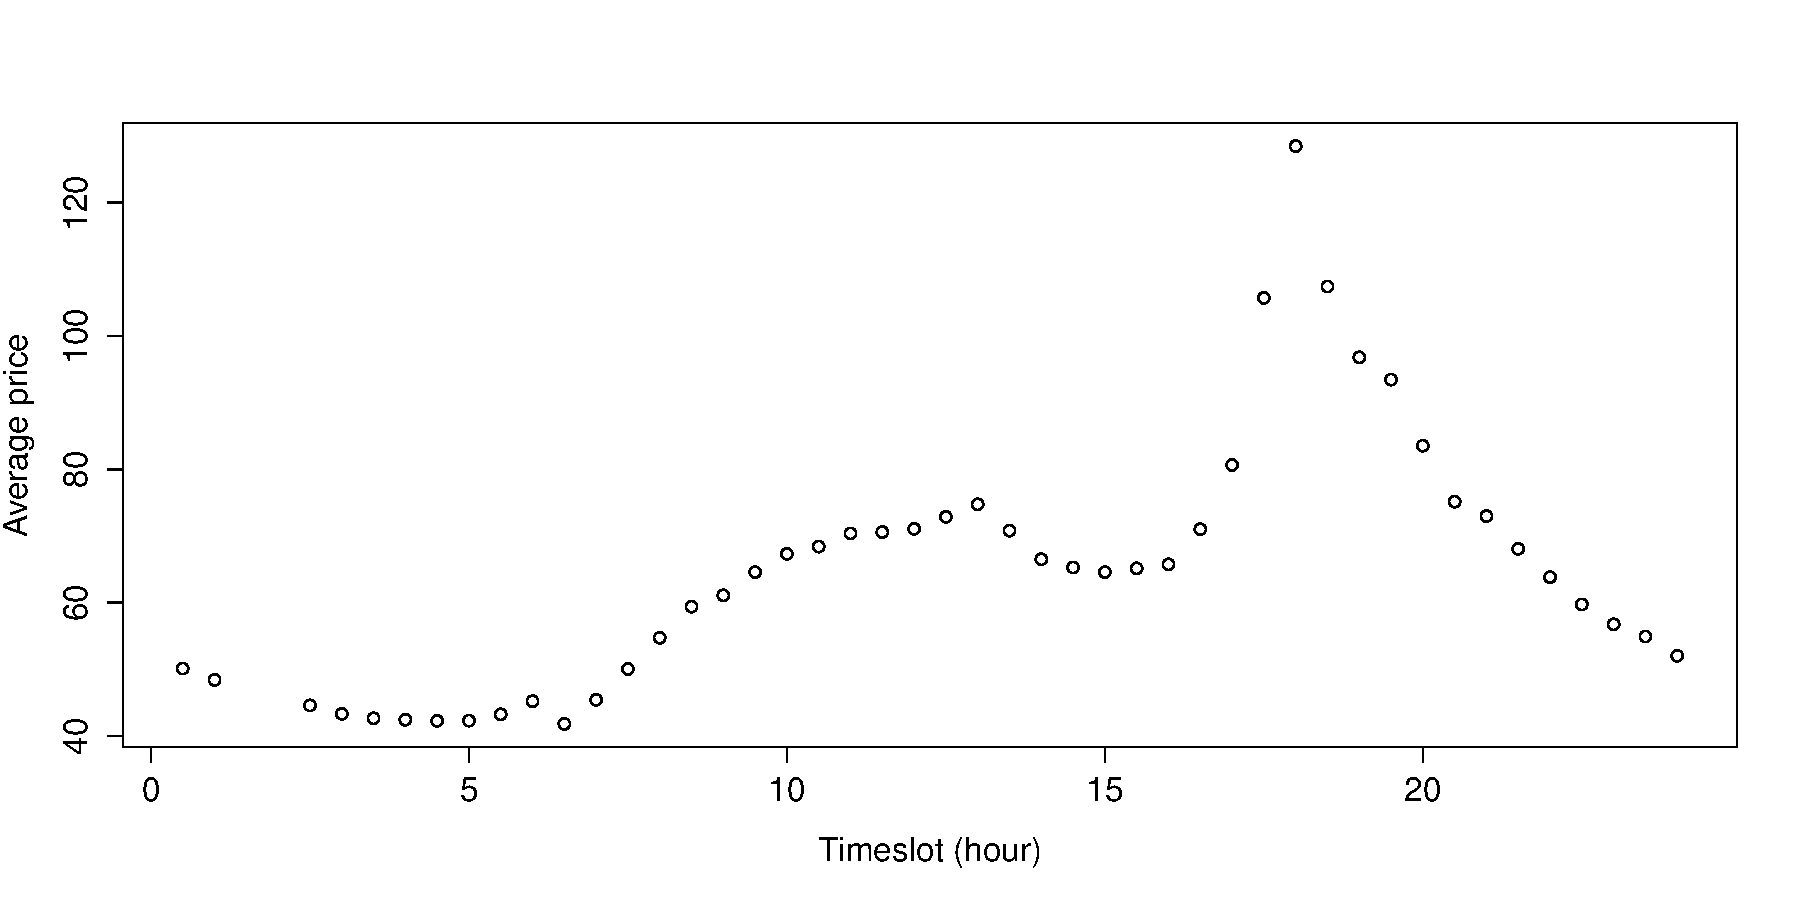
\includegraphics[width=.8\textwidth]{img/timeslot_averageprice.pdf}
	\caption{The average price during the day, measured per half hour.}
	\label{fig:timeslot_average}
\end{figure}

We can see a clear peak of price of energy at 18h00. This makes sense intuivitely. The energy consumption of consumers is the highest at that time and the energy market follows the simple principles of supply and demand. To make the relation between \verb|PeriodOfDay| and the actual price more linear, we transform it to a new feature \verb|PeriodsToPeak|. This new feature is the number of periods between the current period and the peak at 18h00. At 10h00 in the morning for example, the \verb|PeriodsToPeak| value is 16. This new feature achieves a better correlation with the actual price than just the raw period of the day.
\begin{verbatim}
prices.PeriodsToPeak          -0.413861750
\end{verbatim}
In conclusion, our linear regression model uses the following three features: \verb|SystemLoadEA|, \verb|SMPEA| and \verb|PeriodstoPeak|.

\subsection{Learning approach}
To estimate prices, we perform linear regression on the selected features discussed above. As such, the parameters of our estimation consist of a set of weights and an intercept. This intercept can be seen as just another weight that gets multiplied with a constant input of $1$.

\subsection{Integration}

\begin{figure}
	\centering
	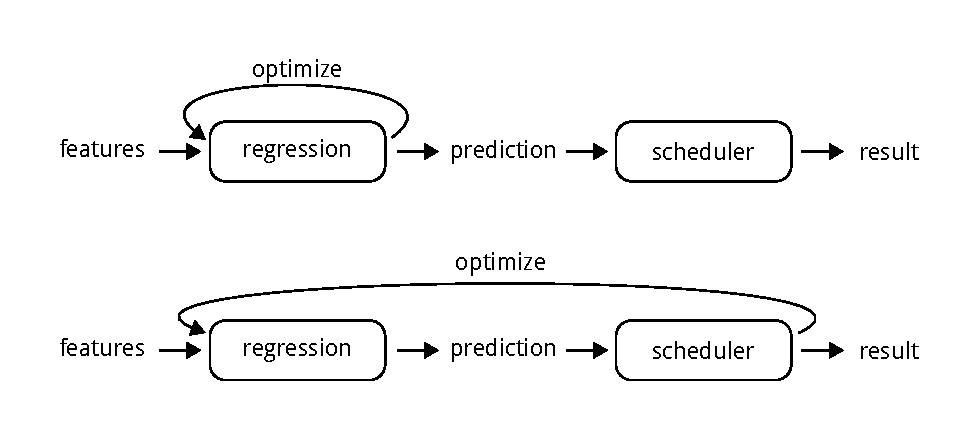
\includegraphics[width=\textwidth]{img/feedback.pdf}
	\caption{Difference between the prototype (top) and our integrated approach (bottom).}
	\label{fig:feedback}
\end{figure}

We have integrated the learning and scheduling phase by iteratively adapting the regression parameters to produce a more cost-efficient schedule. This is different from the standard approach, where the regression parameters are chosen to estimate the actual prices as closely as possible. A schematic overview of this can be seen in figure \ref{fig:feedback}. However, a better price estimate may not necessarily result in a better schedule\cite{ifrim2012properties}.

Since the actual energy prices for each day are not known at the time of scheduling, we cannot use them to evaluate generated schedules to select the best one. To overcome this problem, we introduce an assumption: the feature values and actual prices of the day before the current day are representative for the current day with respect to the scheduling. We then pose the question: "what would yesterday have been the best possible model for the load of today". We answer this question by searching locally for weights that result in a schedule which minimizes the total cost. To perform this search, we use a hill climber. The hill climber is initialized with weights learned from performing ordinary least-squares on a set of history days (by default 30). During each iteration, the weights are modified and a new schedule is generated using MiniZinc. Note that, while the constraint problem solved corresponds to the load \emph{of the current day}, the feature values \emph{of the day before} are used during the training. The resulting schedule is then evaluated with the actual price of the day before. 

\section{Experiments}
%results and discussion (of interesting experiments you did
Table \ref{tab:results} shows results for the prototype, a linear regression model using only \verb|SystemLoadEA|, \verb|SMPEA| and \verb|PeriodstoPeak|, and our model that trains a set of weights on the previous day (we try 10 and 100 random weight mutations per day). We do not report execution times because the time needed to execute our python scripts is negligible compared to the execution time of minizinc optimizing the constraint problem for forecasted prices. It takes about 1.5 seconds to generate a schedule for a day from load1, but the execution time quickly rises when using different loads. A day from load4 for example takes $\pm 10$ seconds to schedule and a day from load8 takes $\pm 90$ seconds to schedule. Because of our limited computing resources, days from load8 are only scheduled by our basic linear regression model and not our full pipeline with the feedback loop.

\begin{table}
	\begin{tabular}{lllllr}
		startday & load &optimal & prototype & lin reg & pipeline\\
		2013-02-01 & load1 & 22,677,406& 22,955,395 & 22,906,306 & 22,907,791\\
		2013-05-01 & load1 & 21,534,652& 21,961,676 & 22,022,949 & 22,544,988\\
		2013-08-01 & load1 & 23,052,956& 23,325,484 & 23,310,270 & 23,399,398\\
		2013-11-01 & load1 & 23,782,343& 24,358,360 & 24,360,228 & 24,347,961\\
		2013-02-01 & load8 & x& 61,833,570 & x & N/A\\
		2013-05-01 & load8 & x& 67,003,304 & x & N/A\\
		2013-08-01 & load8 & x& 68,446,485 & x & N/A\\
		2013-11-01 & load8 & x& 64,945,087 & x & N/A\\
	\end{tabular}
	\caption{The performance of our models compared to the performance of the prototype and the optimal schedule for different combinations of loads and starting days.}
	\label{tab:results}
\end{table}
Our basic linear regression model has comparable results to the prototype and our full pipeline is a bit worse. We can conclude that when dealing with limited computing resources, it is probably better to focus on accurate price predictions. A simple attempt at optimizing the full pipeline actually gave worse results and takes a very long time to train. 


\section{Conclusion}
%conclusions and future work (if you had more time, you would investigate...);

%in solving an energy-aware scheduling problem. 

A simple analysis of the energy price data indicated that there are only three relevant features. One of these features: \verb+PeriodOfDay+, has been transformed into a new feature \verb+PeriodsToPeak+ which is more correlated to the actual price. A linear regression model trained using only these three features performs comparable to the prototypical approach that uses all available features.

We have furthermore introduced an approach that uses local search to closely integrate the learning and scheduling phases. Instead of approximating the actual price of each day, our approach directly minimizes the total cost of the resulting schedules. Our experiments show that this approach is not really advantageous over using simple linear regression. If this approach were to be adopted in practice, we suggest minimizing the schedule cost for more than one day and replacing the MiniZinc scheduler with a heuristic method during training time. 

\bibliographystyle{plain}
\bibliography{references.bib}

\end{document}